\mychapter{5}{Signal extracted on DATA}
\label{sec:unchapitre}

In this section will be extracted \textgamma+jet event purity on real data.
First we must establish PDF for signal (MC simulation) and background (real data in sideband), the analysis will be
performed on the $p_T^\gamma$ range [ 40 GeV ; 3000 GeV ] divided in 12 bins.

\section{Probability Density Function parametrization}

PDF are established using the ROOFit framework of ROOT using MC simulation for signal and real data in the sideband for the background.
Then MVA response for data in the signal region is expressed as : 

\begin{equation}
MVA(Data_{signal}) = a*PDF(MC_{signal}) + b*PDF(Data_{sideband})
\end{equation}

With : 
\begin{itemize}
	\item $MVA(Data_{signal}) :=$ the MVA response for Data in the signal region.
	\item $PDF(MC_{signal}) :=$ PDF for MC in the signal region.
	\item $PDF(Data_{sideband}) :=$ PDF for Data in the sideband. 
	\item $a :=$ number of signal events.
	\item $b :=$ number of background events. 
\end{itemize}

%\begin{figure}[h!]
%\centering
%    
\includegraphics[width=0.5\textwidth]{coming_soon}
%    \caption{Example of PDF parametrization for $p_T^\gamma \in [ 75 GeV ; 230 GeV ]$}
%    \label{coming_soon}
%\end{figure}

\section{Fit on Data}

With the PDF established in the previous section we want to extract values of the parameters $a$ and $b$ representing
signal and background proportion in the sample. For this analysis we will perform a maximum likelihood estimation for
each $p_T^\gamma$ range that has been defined. (fig \ref{pt_5_dataset}) show for example the fit perfomed for
$p_T^\gamma \in [ 75 GeV ; 230 GeV ]$

\begin{figure}[h!]
\centering
    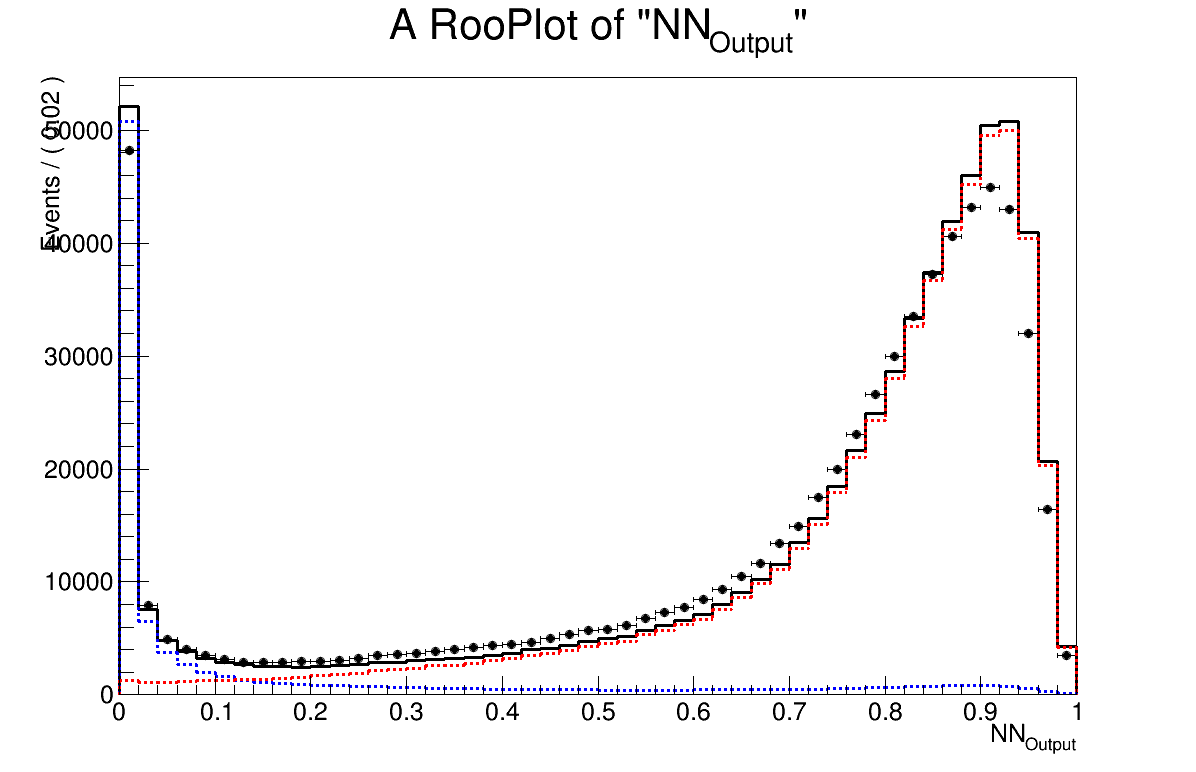
\includegraphics[width=0.7\textwidth]{pt_5_dataset}
    \caption{Example of a maximum likelihood fit performed for $p_T^\gamma \in [ 75 GeV ; 230 GeV ]$, showing background
    PDF (blue dotted line) signal PDF (red dotted line) and fit result (solid black line) superimposed with real data (black dot).}
    \label{pt_5_dataset}
\end{figure}

\subsection{Pulls distribution cross-check}

In order to perform a cross-ckeck of the maximum-likelihood we generate a pull distribution for each $p_T^\gamma$ range.

\begin{figure}[h!]
\centering
    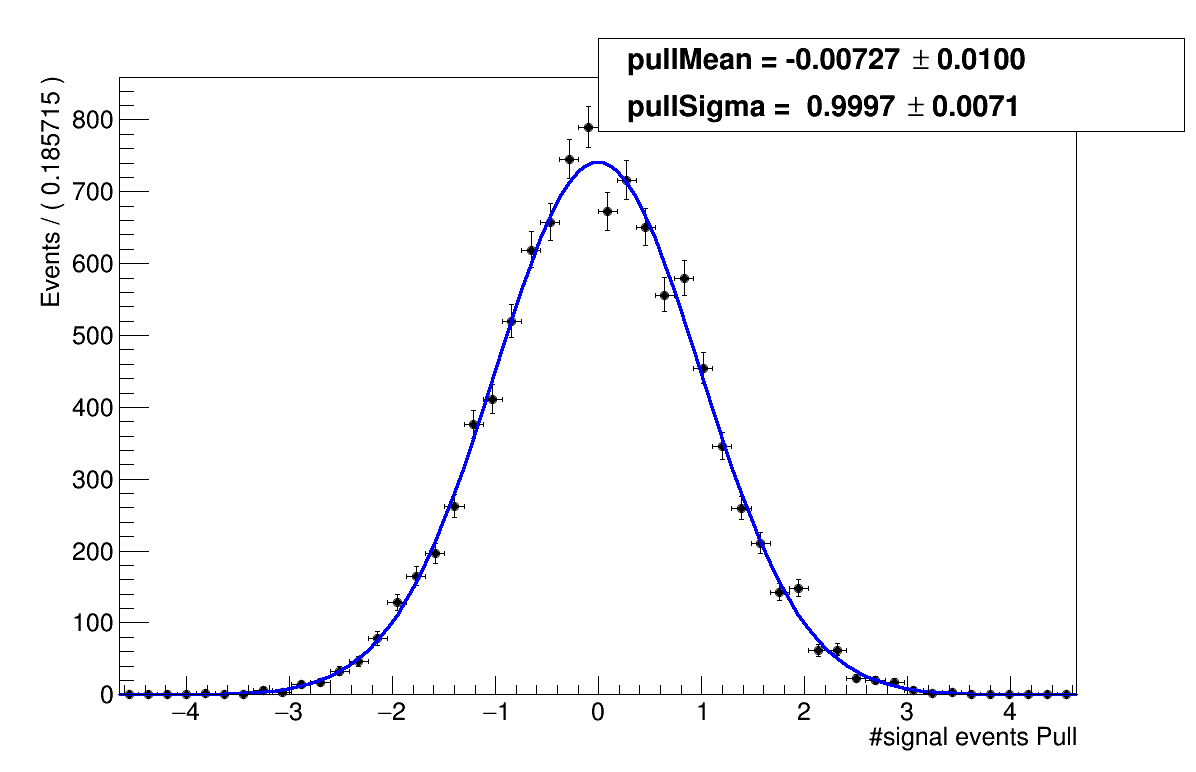
\includegraphics[width=0.7\textwidth]{pull_plot}
    \caption{Example of a pull plot performed for $p_T^\gamma \in [ 75 GeV ; 230 GeV ]$, showing background PDF (dotted
    blue line) signal PDF (dotted red line) and fit result (solid black line) superimposed with real data (black dot).}
    \label{pull_plot}
\end{figure}

\subsection{\textgamma+jet events purity}

Finally the estimated parameters representing background and signal proportions are used to construct the \textgamma+jet
events (signal) purity function of the $p_T^\gamma$ (fig. \ref{purity}).
\begin{figure}[h!]
\centering
    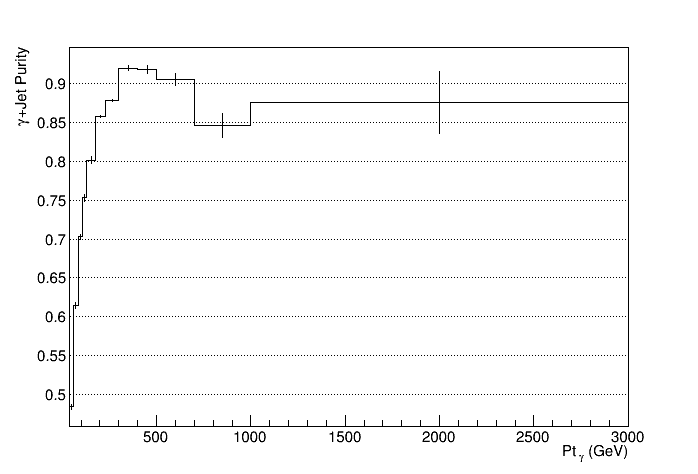
\includegraphics[width=0.7\textwidth]{purity}
    \caption{\textgamma+jet purity function of $p_T^\gamma \in [ 40 GeV ; 3000 GeV ]$ evaluated with the ANN, showing background PDF (dotted
    blue line) signal PDF (dotted red line) and fit result (solid black line) superimposed with real data (black dot).}
    \label{purity}
\end{figure}

%%% Local Variables: 
%%% mode: latex
%%% TeX-master: "isae-report-template"
%%% End: 
